\chapter{Introdução}

\section{Objetivos}
Descrever a mudança de paradigma no campo de aprendizado de máquina através do advento das técnicas de aprendizado profundo, chamadas \textit{deep learning}.  Além disso, busca­-se exemplificar o uso dessas técnicas com um problema prático e assim demonstrar resultados do estado da arte para classificação de imagens e localização de objetos.
 
\section{Motivação}
Na década de 1970 as redes convolucionais já estavam sendo desenvolvidas, porém os algoritmos de treinamento ainda eram precários e a técnica acabou sendo abandonada em detrimento de técnicas superficiais, como \textit{Support Vector Machines}.

Com o aumento drástico do poder de processamento essas redes ultrapassaram seus predecessores e ganharam destaque novamente após o trabalho de Hinton \cite{hintonDL} em 2006, que estabeleceu uma base sólida para o treinamento de grandes redes convolucionais. Essa contribuição mudou o paradigma do aprendizado de máquina no que se refere à extração de características e se mostra ainda hoje como estado da arte. 

Destacam-se aplicações em visão computacional, onde após a introdução da técnica os trabalhos seguintes continuaram aperfeiçoando a técnica para atingir níveis melhores de classificação. Ainda, a recente vitória do algoritmo \textit{AlphaGo}, baseado em aprendizado por reforço, sobre o campeão mundial de Go trouxe a atenção do grande público para essa tecnologia.

O recente investimento de gigantes como \textit{Google}, \textit{Facebook} e \textit{Yahoo} nesse segmento em conjunto com a grande quantidade de artigos inovadores no tema demonstram que essa técnica é de grande relevância e permitirá explorar problemas complexos de grande interesse para a indústria e academia brasileiras.

\section{Metodologia}
A metodologia consiste em revisar a literatura da área de forma a compreender as principais estruturas envolvidas, especialmente as redes convolucionais, suas conexões e mudanças em relação aos métodos tradicionais.

Após a revisão, um problema de localização de objetos é introduzido. Trata-se da tecnologia de detecção de pessoas que é empregada em um ambiente industrial para garantir a segurança dos funcionários. Nessa indústria existe uma ponte rolante utilizada para carregar peças de até centenas de kilogramas em torno do ambiente industrial. Dessa forma, é necessário garantir que durante essa manipulação não existam colaboradores debaixo da mesma. Propõe-se então três soluções para esse problema a partir de imagens de profundidade geradas por uma câmera stereo.

A primeira é fundamentada nos métodos tradicionais de visão computacional e aprendizado de máquina. Divide-se o algoritmo em obtenção de candidatos à pessoas e posterior extração de características, desenvolvida manualmente, e classificação através de \textit{Support Vector Machines}.

Em seguida, propõe-se um método que emprega o mesmo algoritmo tradicional de obtenção de candidatos porém utiliza métodos de aprendizado profundo para encontrar de maneira automática um descritor de caracterísitcas específico para o conjunto de dados do problema. A classificação se dá nas camadas finais da rede profunda.

A terceira solução é concebida utilizando-se integralmente soluções de aprendizado profundo. Uma rede de convolução é utilizada e recebe como entrada a imagem completa do ambiente industrial. A saída é uma máscara indicando a posição das pessoas encontradas na imagem. Essa rede é treinada utilizando um amplo conjunto de quadros e algortimo de propagação reversa de erros.

Tendo implementado os métodos e de posse de um dataset grande o suficiente para o treinamento das redes profundas, espera-se avaliar a performance de cada opção proposta e verificar qual a melhor solução, além de observar o impacto da utilização das redes profundas em diferentes etapas do sistema.

\section{Definições}
Segundo Arthur Samuel, aprendizado de máquina é o ramo da inteligência artificial que estuda técnicas que possibilitam um computador realizar uma tarefa sem ser explicitamente programado para desempenhá-la. 

Mitchell (1997) define: "Se diz que um computador aprende com uma experiência $E$ com respeito a uma tarefa $T$ e medida de performance $P$ a medida que a performance medida por $P$ medida em uma tarefa $T$ progride com a experiência $E$". 

Entre as tarefas pode-se citar classificação, em que uma amostra deve ser atribuída a uma das classes apresentadas; regressão, em que uma amostra deve ser mapeada em um valor real; síntese, onde o algoritmo deve gerar novas amostras que sejam similares às de entrada.

As medidas de performance são específicas da tarefa em questão e seu uso deve variar com a aplicação. Para conjuntos de dados simples e balanceados uma medida comum a classificadores é a Exatidão Geral (EG), razão do número correto de classificações pelo número total. Porém a Exatidão Específica (EE), razão das classificações corretas pelo número total da classe, fornece maiores indicativos sobre o potencial discriminativo do algoritmo. Para problemas de regressão podem ser adotadas as medidas de erro médio quadrático.

As experiências são o conjunto de dados que o algoritmo utiliza para aprender, aqui também chamado de \textit{dataset}. Esse conjunto de dados é dito supervisionado quando possui um indicador da classe que cada amostra pertence ou o valor esperado para aquela amostra, no caso de regressão. Para um conjunto não supervisionado, espera-se aprender mais sobre a distribuição dos dados. Isso permite, por exemplo, detectar amostras anômalas e dividir o conjunto de dados em grupos (\textit{clusters}) que apresentem alguma similaridade estrutural.

Uma experiência, também chamada de exemplo ou amostra, é uma coleção de descrições, obtida através de um descritor de características. Essa descrição é obtida através de um processo que pode mensurar alguma grandeza específica de algum objeto ou evento. Para o campo de imagens são comuns descritores de borda e histograma de cores. Em geral, um descritor busca obter uma representação compacta e discrimantiva entre as amostras. 

%Adicionar imagem representando descritores 

\section{Métodos clássicos}
O problema de classificação de imagens é um clássico no campo de visão computacional e requer aprendizado de máquina. Uma abordagem tradicional consiste nos seguintes passos.
	\begin{enumerate}
	\item Identificar uma região de interesse no caso de uma imagem com múltiplos objetos.
	\item Utilizar um extrator de características para descrição da imagem.
	\item Introduzir a amostra, proveniente do descritor, em um classificador, obtendo a classe correspondente.
	\end{enumerate}

A escolha do descritor está diretamente ligada com a qualidade do processo de classificação. Um descritor é criado especificamente para uma aplicação e dificilmente pode ser utilizado em outros campos: um descritor para imagens não consegue entender um sinal de áudio. Assim, sua concepção demanda conhecimento e prática de especialistas da área de aplicação. Para um problema de classificação entre imagens de bananas e maçãs, por exemplo, um descritor relacionado a cor teria maior relevância do que a representação completa dos pixels das imagens.

% SVM
Após ter uma representação adequada das experiências escolhe-se o tipo do classificador. O modelo de \textit{Support Vector Machines} é bastante utilizado pois possui representação e uso simplificado e demonstrou bons resultados ao tratar amostras de dimensões medianas (ordem de centenas) com um dataset pequeno (ordem de milhares de amostras) sem ajuste fino. Seu modelo consiste em encontrar um hiperplano de separação entre classes ótimo, no sentido de maximizar a distância entre as amostras e o hiperplano. As amostras mais próximas do hiperplano são chamadas vetores suportes.

\begin{figure}[h]
\caption{Hiperplano ótimo para separação das classes}
\centering
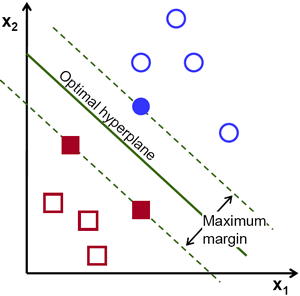
\includegraphics[width=0.5\textwidth]{svm/svm-hyperplane}
\label{fig:svm-hyperplane}
\end{figure}

Para amostras com distribuição complexa a possibilidade de não existir um hiperplano que consiga separar o conjunto satisfatóriamente é grande. Para resolver esse problema emprega-se uma função que mapeia essas amostras para um espaço de maior dimensionalidade em que as classes sejam linearmente separáveis. Na prática, entretanto, não se calcula as coordenadas da amostra transformada no novo espaço, mas uma técnica chamada \textit{kernel trick} em que o produto interno dessa amostra transformada é obtida diretamente através da amostra original, o que permite que o método seja escale mais facilmente.

\begin{figure}[h]
\caption{Exemplo de mapeamento para obter um classes linearmente separáveis}
\centering
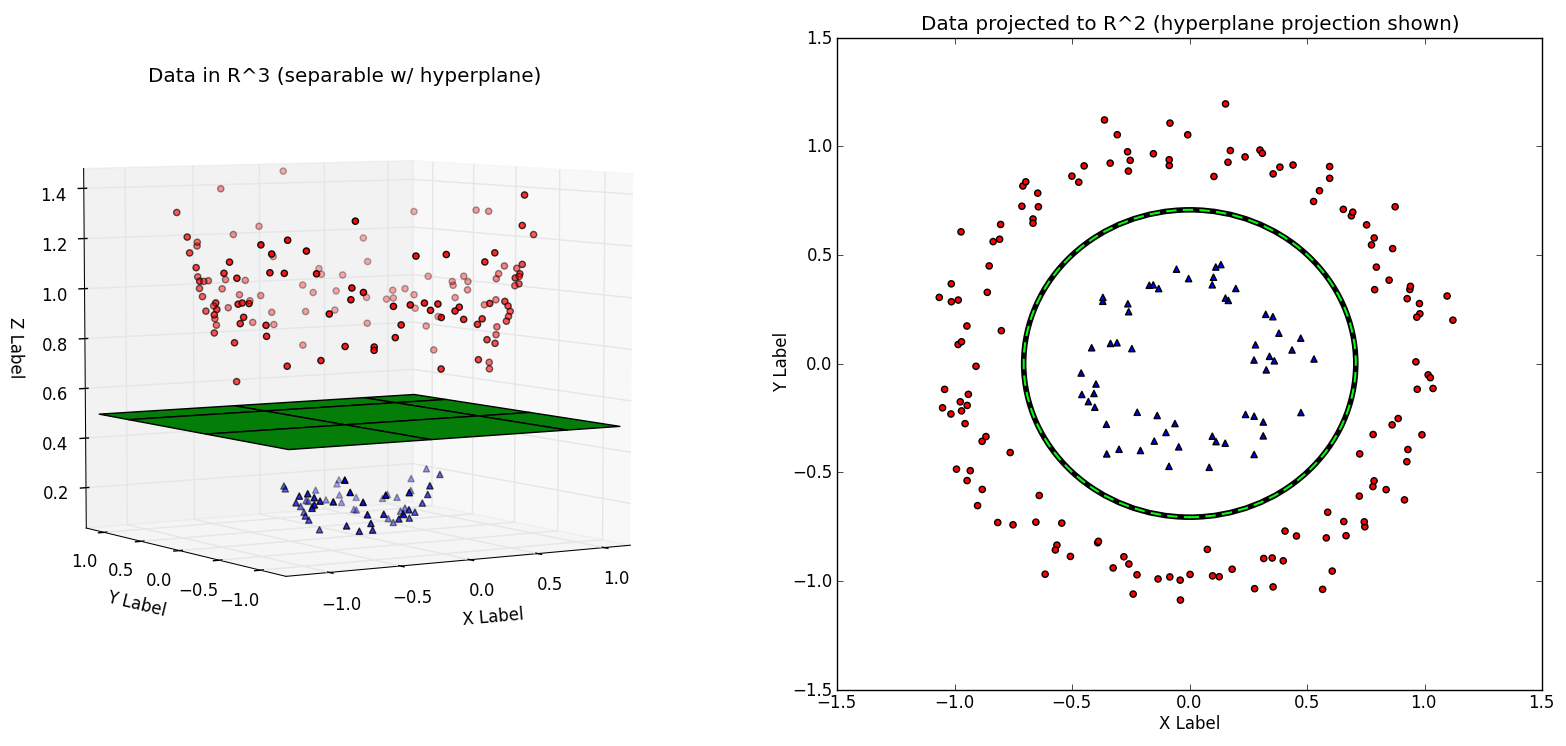
\includegraphics[width=0.8\textwidth]{svm/svm-kernel}
\label{fig:svm-kernel}
\end{figure}

Para classificações não-binárias pode-se adotar a estratégia \textit{one-vs-one} em que um classificador binário é utilizado para cada par de classes e o resultado é obtido pela classe que for mais votada entre os classificadores binários.

\section{Aprendizado profundo}
\section{Caracterização da aplicação}

